\subsubsection{JIT Emulator}
\label{section:perf-jit}

\autoref{figure:jit-vs-interpreter} shows the execution time of all tests for the JIT emulator vs the interpreter. It can be seen that, in general, the JIT emulator is able to significantly outperform the interpreter for longer tests, yet performs poorly on shorter tests. More specifically, the execution time appears to have a `floor' of $\sim10\si{\micro\second}$ for the JIT emulator. For very short tests, the execution time for the interpreter falls while the JIT is not able to overcome this barrier. This property will be explored further in more depth.

\begin{figure}[H]
    \centering
    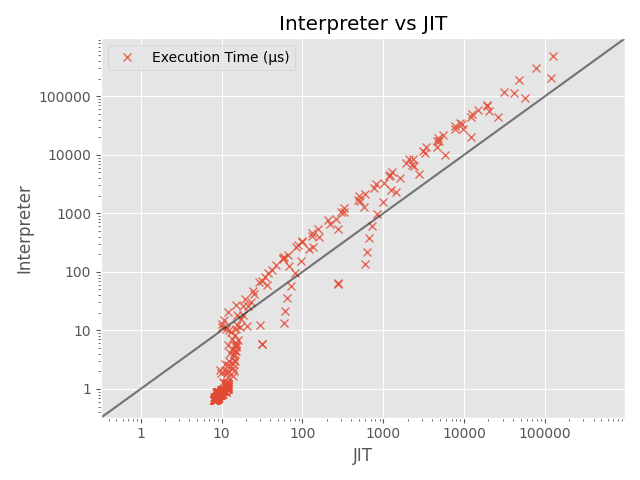
\includegraphics[scale=0.75]{output/graphs/scatter/vs/JIT-vs-Interpreter-time.png}
    \caption{Execution time of all tests for the JIT emulator vs the interpreter.}
    \label{figure:jit-vs-interpreter}
\end{figure}

To investigate the performance characteristics of the JIT emulator, one factor of interest is the hotness of the tests; the performance vs hotness is shown in \autoref{figure:jit-hotness}.

\begin{figure}[H]
    \centering
    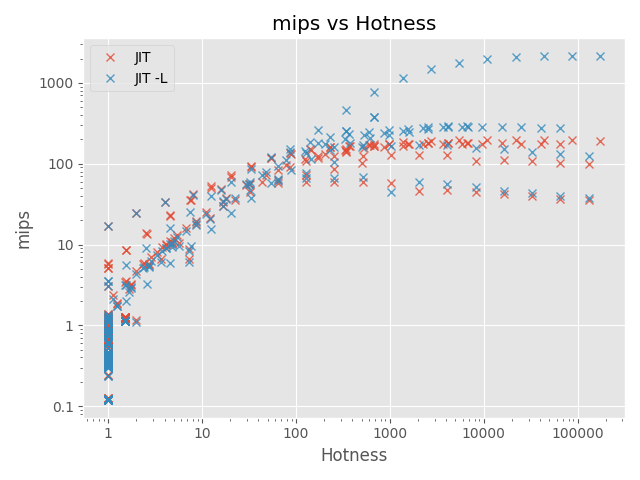
\includegraphics[scale=0.75]{output/graphs/scatter/jit/hotness.png}
    \caption{Performance (mips) vs hotness for all tests run on the JIT emulator.}
    \label{figure:jit-hotness}
\end{figure}

A very clear positive relationship between the hotness of a test and the performance under the JIT can be seen. As the hotness increases the performance also tends to increase, up until a point at which the performance `saturates'. This behaviour occurs because hotter blocks are run more frequently, and thus the initial compilation cost becomes proportionally smaller. After a point, however, this initial cost becomes irrelevant and the execution time of the block becomes the dominating factor; since being hotter doesn't reduce this (excluding caching benefits) the performance increase saturates. It can be seen that \texttt{JIT -L} saturates later at a much higher performance.

\autoref{figure:primal-mips} shows the performance of the \texttt{primal(n)} test suite on the JIT emulators. The test suite consists primarily of a single hot loop, and thus we should expect to see similar performance characteristics.

\begin{figure}[H]
    \centering
    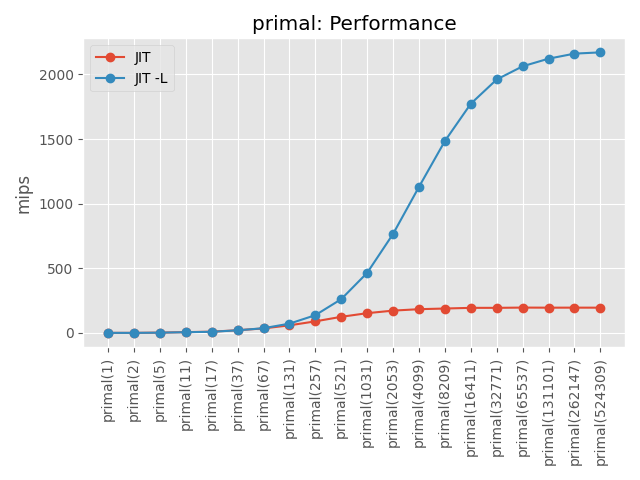
\includegraphics[scale=0.75]{output/graphs/tests/jit/primal/mips.png}
    \caption{Performance in mips of the primal test suite run on the JIT emulator.}
    \label{figure:jit-primal-mips}
\end{figure}

It is evident that as \texttt{n} increases the performance of both SUTs increases significantly, however \texttt{-L} saturates later at a much higher performance, roughly $\sim 10\times$ higher. \texttt{primal(n)} is a best case scenario for \texttt{JIT -L} as it is a very hot loop with no memory operations; this allows it the emulator to operate extremely fast once all the overheads have been amortized.

\begin{figure}[H]
    \centering
    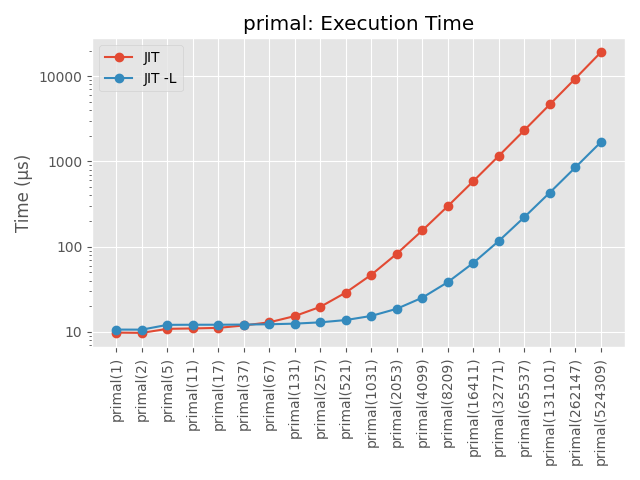
\includegraphics[scale=0.75]{output/graphs/tests/jit/primal/time.png}
    \caption{Execution time of the primal test suite run on the JIT emulator.}
    \label{figure:jit-primal-time}
\end{figure}

The effects of the fixed costs and initial overheads is much more present in the execution times as illustrated by \autoref{figure:jit-primal-time}. It can clearly be seen that for small \texttt{n} the execution time remains relatively constant at $\sim10\si{\micro\second}$. This would indicate that, under the circumstances tested, the JIT had a fixed cost of $\sim10\si{\micro\second}$. As \texttt{n} increases the execution time becomes more significant than the overhead, and we start to see the total execution time rise significantly.

While \texttt{-L} clearly gives superior results for hotter and more performance intensive tasks, we would expect lighter workloads to suffer; \texttt{-L} increases the overheads due to the relinking process, and the increased execution performance likely won't have time to make up for it.

\begin{figure}[H]
    \centering
    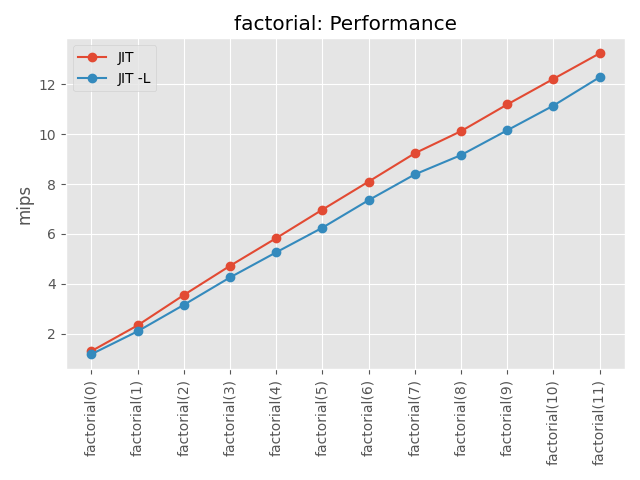
\includegraphics[scale=0.75]{output/graphs/tests/jit/factorial/mips.png}
    \caption{Performance in mips of the factorial test suite run on the JIT emulator.}
    \label{figure:jit-factorial-mips}
\end{figure}

The test suite \texttt{factorial(n)} can only be used for small \texttt{n} due to how explosively $n!$ increases with $n$; the performance for this test suite is shown in \autoref{figure:jit-factorial-mips}. It can be seen that \texttt{-L} causes a slight, but consistent drop in performance compared to the standard vanilla \texttt{JIT} configuration. The performance in these scenarios is very poor even without \texttt{-L}, so this is not a compelling reason to disable \texttt{-L} as the high performance in heavier workloads more than makes up for it.

A more general picture can be seen by comparing the execution time of all tests between \texttt{JIT -L} and the standard \texttt{JIT} as shown by \autoref{figure:jit-l-vs-jit}. It can be seen that most tests perform the same or better with \texttt{-L} enabled, with some tests performing orders of magnitude better.

\begin{figure}[H]
    \centering
    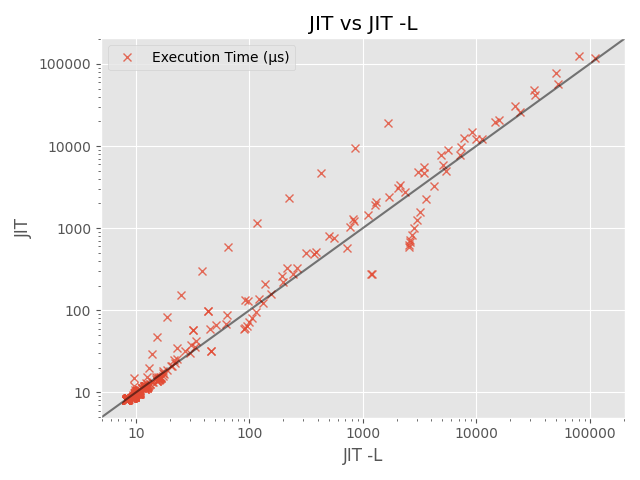
\includegraphics[scale=0.75]{output/graphs/scatter/vs/JIT -L-vs-JIT-time.png}
    \caption{Execution time of all tests for \texttt{JIT -L} vs \texttt{JIT}.}
    \label{figure:jit-l-vs-jit}
\end{figure}

We can then compare \texttt{JIT -L} to the interpreter as shown in \autoref{figure:jit-l-vs-interpreter}. For short tests, \texttt{JIT -L} loses to the interpreter just as the standard \texttt{JIT} does (as shown by \autoref{figure:jit-vs-interpreter}). The clear difference with \texttt{-L} enabled is that the tests that already perform well without \texttt{-L} now perform even better, in some orders of magnitudes better. This is further reason to believe that \texttt{-L} is a beneficial feature despite not globally improving performance.

\begin{figure}[H]
    \centering
    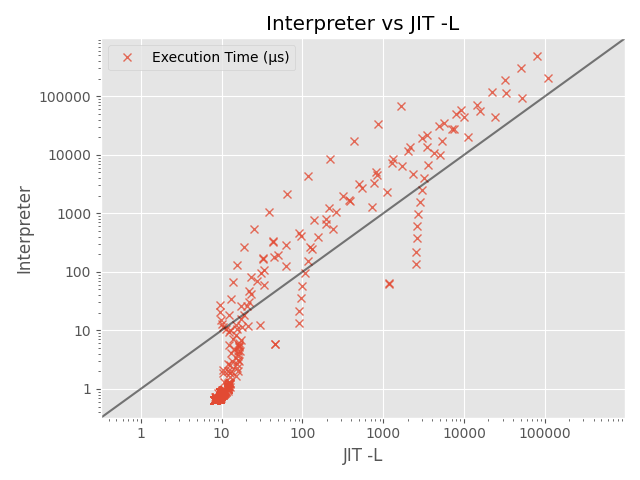
\includegraphics[scale=0.75]{output/graphs/scatter/vs/JIT -L-vs-Interpreter-time.png}
    \caption{Execution time of all tests for \texttt{JIT -L} vs the interpreter.}
    \label{figure:jit-l-vs-interpreter}
\end{figure}

Another metric of interest is the compilation inefficiency. A high compilation inefficiency would indicate that many host instructions are compiled to emulate a few source instructions; generally speaking, the fewer instructions used the better. Not only should they be faster to compile, as generating instructions has an associated overhead, but execution performance should also increase due to better cache utilisation. Having said this, there are many other factors at play such as the instructions themselves and how often they are executed, so we should not expect a strict relationship between compilation inefficiency and performance.

\begin{figure}[H]
    \centering
    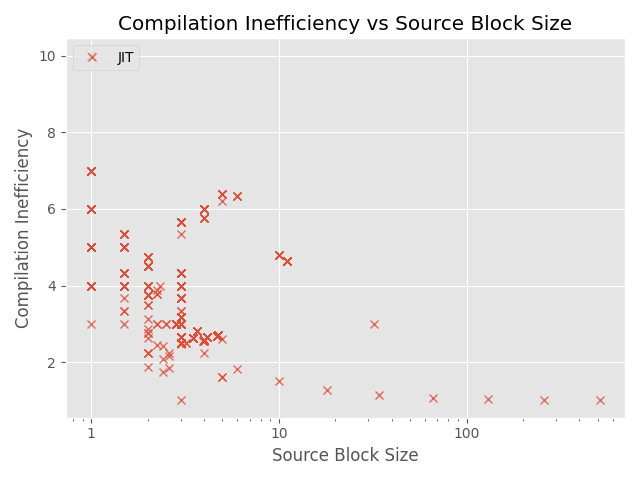
\includegraphics[scale=0.75]{output/graphs/scatter/single/jit/c-efficiency-vs-hotness.png}
    \caption{Compilation inefficiency vs average source block size for all tests.}
    \label{figure:jit-c-inefficiency-size}
\end{figure}

\autoref{figure:jit-c-inefficiency-size} shows the relationship between the average source block size and the compilation inefficiency. From this graph it is very clear that as the source block size increases, the compilation inefficiency falls. This is to be expected as each compiled block includes some setup and teardown instructions, and thus the bigger the block the smaller effect these have. Due to this, it is ideal that the block partitioner produces the largest source blocks possible.

\begin{figure}[H]
    \centering
    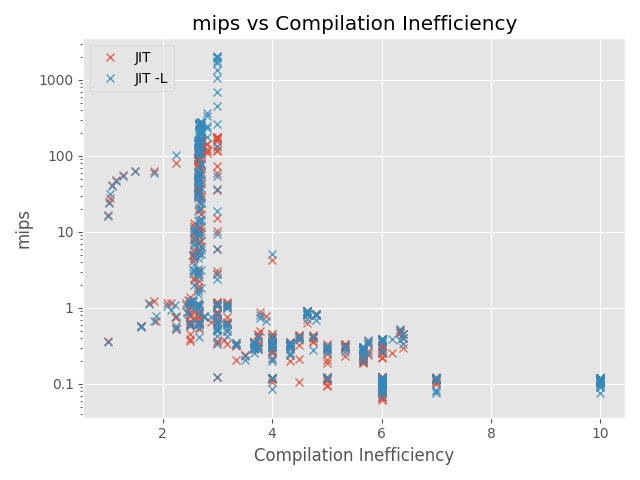
\includegraphics[scale=0.75]{output/graphs/scatter/jit/c-efficiency-vs-mips.png}
    \caption{Performance (mips) vs compilation inefficiency for all tests.}
    \label{figure:jit-c-inefficiency-mips}
\end{figure}

More importantly, however, if the relationship between compilation inefficiency and performance. \autoref{figure:jit-c-inefficiency-mips} shows that there is quite a clear reciprocal relationship between the performance and the compilation inefficiency; as compilation inefficiency rises the performance drops drastically for both \texttt{JIT} and \texttt{JIT -L}.

The ideal configuration found for the JIT emulator is detailed in \autoref{tbl:jit-optimal}

\begin{table}[H] 
    \centering
    \begin{tabular}{l|c}
        \toprule
        Option & Value \\
        \midrule
        \texttt{-L} & \cmark \\
        \bottomrule
    \end{tabular}
    \caption{Optimal configuration found for the JIT emulator.}
    \label{tbl:jit-optimal}
\end{table}